\chapter{बैटरियाँ, ईंधन सेल और विद्युत-अपघटन}\label{ch:b2:batteries-electrolysis}

अयस्क से प्राप्त हर किलोग्राम ऐलुमिनियम में लगभग \qty{13}{kW.h}
बिजली लगती है; एक किलोग्राम कबाड़ को पिघलाने में, सिद्धांततः, केवल वे
\qty{0.3}{kW.h} लगते हैं जो उसे गलनांक तक गर्म करके पिघला दें। अंतर
\omterm{def:b2:batteries-electrolysis:electrolysis}{विद्युत-अपघटन} सेलों की एक लंबी पंक्ति का कार्य है, जिनमें से हर एक कुछ वोल्ट पर
पिघले लवण से होकर लाखों ऐम्पियर प्रवाहित करता है। बैटरी उलटी दिशा में
चलती है: एक स्वतः अभिक्रिया धारा चलाती है।
\cref{ch:b2:current-potential-curves} के \omterm{def:b2:current-potential-curves:ie-curve}{धारा--विभव वक्रों} से दोनों
एक ही आरेख पर पढ़े जाते हैं, और अम्ल में घुलता ज़िंक का एक टुकड़ा भी।
% ledger: hT:Al_l.933, aw:Al

\begin{recall}
\Cref{ch:b2:cell-thermodynamics}: $\Delta_r G = -nFE$, अधिकतम कार्य,
\omterm{def:b2:cell-thermodynamics:faraday}{फ़ैराडे स्थिरांक}। \Cref{ch:b2:current-potential-curves}: \omterm{def:b2:current-potential-curves:ie-curve}{धारा--विभव
वक्र}, तीव्र और \omterm{def:b2:current-potential-curves:fast-slow}{मंद निकाय}, \omterm{def:b2:current-potential-curves:overpotential}{अधिविभव}, सीमांत धाराएँ, जल की
भित्तियाँ। \Cref{ch:b2:ellingham}: ऐलुमिनियम कार्बन से क्यों प्राप्त नहीं होता। विद्यालय
का खंड: \omterm{def:b2:batteries-electrolysis:electrolysis}{विद्युत-अपघटन}, \omterm{def:b2:batteries-electrolysis:battery}{संचायक}।
\end{recall}

\begin{omfigure}
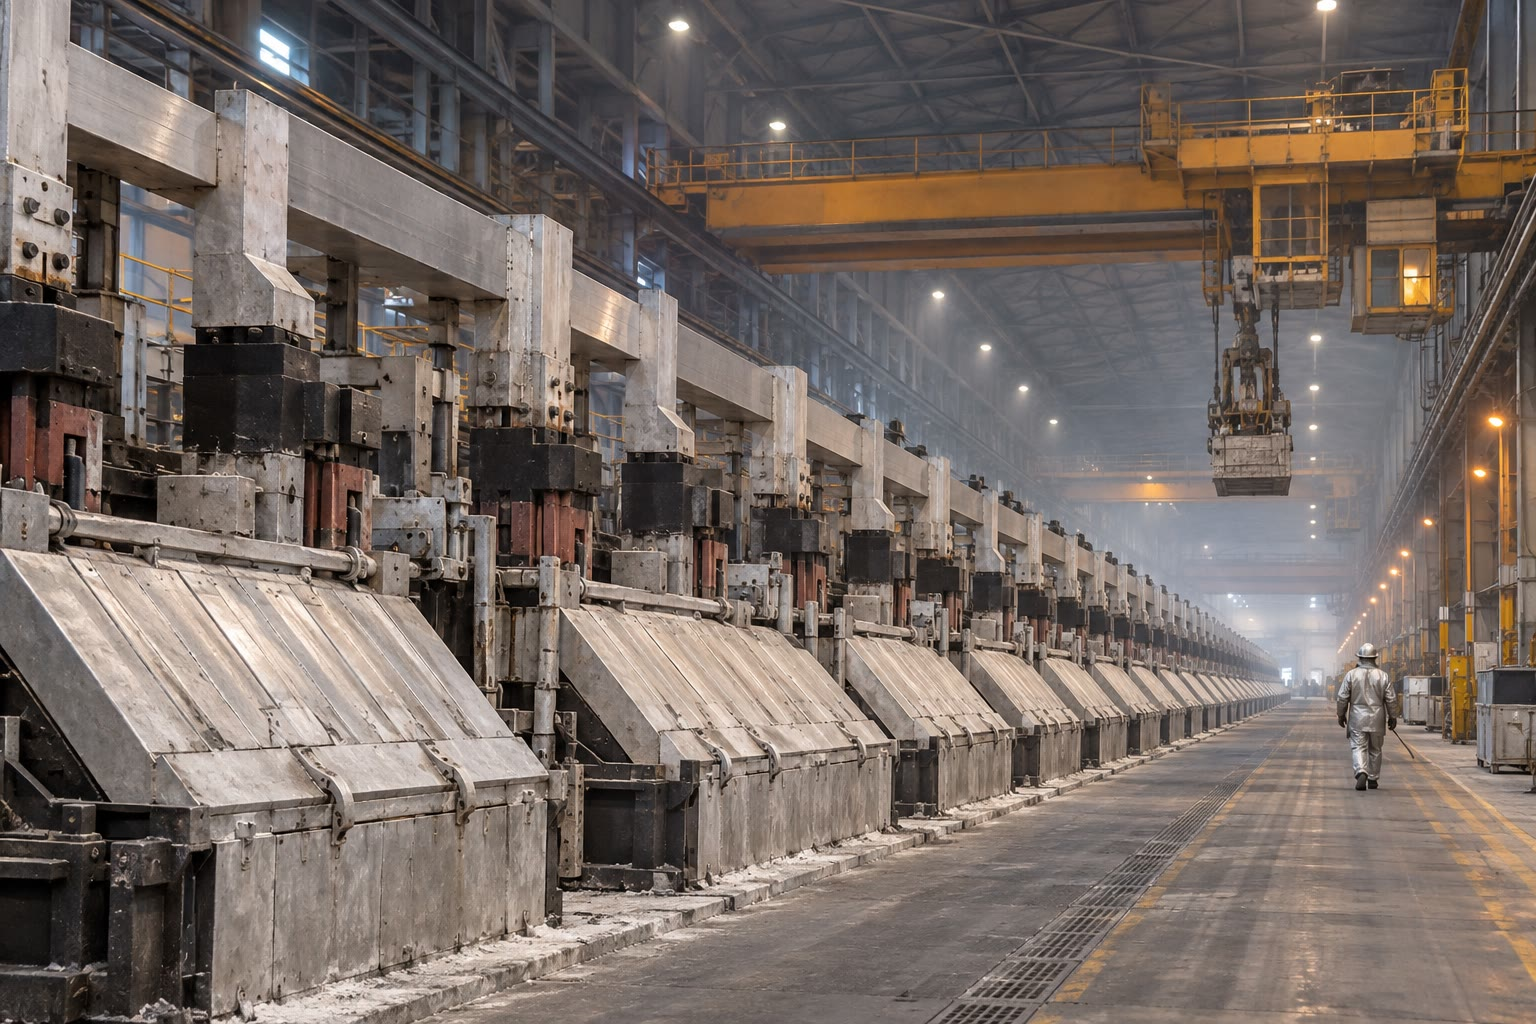
\includegraphics[width=0.62\linewidth]{images/book3/ai/b2-11-potroom.jpg}

{\small ऐलुमिनियम प्रगालक का पॉट-कक्ष: \omterm{def:b2:batteries-electrolysis:electrolysis}{विद्युत-अपघटन} सेलों की एक पंक्ति,
सैकड़ों लंबी, श्रेणी में जुड़ी; ऊपर लगी क्रेन कार्बन
ऐनोडों के जल जाने पर उन्हें बदलती है।}
\end{omfigure}

\section{वक्रों पर पढ़ी गई स्वतः अभिक्रियाएँ}

\begin{definition}[मिश्र विभव]\label{def:b2:batteries-electrolysis:mixed-potential}
जिस इलेक्ट्रोड पर दो भिन्न युग्म अभिक्रिया करते हैं, एक ऑक्सीकृत और एक अपचित,
उसका \emph{मिश्र विभव}\index{मिश्र विभव} वह विभव है जो वह
तब लेता है जब कोई कुल धारा नहीं बहती: तब एक युग्म की \omterm{def:b2:current-potential-curves:ie-curve}{ऐनोडी धारा}
दूसरे की \omterm{def:b2:current-potential-curves:ie-curve}{कैथोडी धारा} के बराबर और विपरीत होती है।
\end{definition}

\begin{proposition}[विलयन में एक धातु]\label{prop:b2:batteries-electrolysis:mixed}
उसे ऑक्सीकृत कर सकने वाले विलयन में डूबी धातु उस विभव $E_m$ पर स्थिर होती है
जहाँ $i_a(E_m) = -i_c(E_m)$, अर्थात् धातु के ऑक्सीकरण की \omterm{def:b2:current-potential-curves:ie-curve}{ऐनोडी धारा}
ऑक्सीकारक के अपचयन की \omterm{def:b2:current-potential-curves:ie-curve}{कैथोडी धारा} को संतुलित करती है; धातु
दर $i_a(E_m)/(nF)$ से घुलती है।
\end{proposition}

\begin{proof}
धातु का एक पृथक टुकड़ा कोई कुल धारा नहीं ले जाता। दोनों अर्ध-अभिक्रियाएँ उसकी
सतह पर एक ही विभव पर होती हैं, इसलिए उस विभव पर उनके वक्रों पर पढ़ी गई
उनकी धाराओं का योग शून्य होता है। \cref{prop:b2:current-potential-curves:current-rate} से
\omterm{def:b2:current-potential-curves:ie-curve}{ऐनोडी धारा} ऑक्सीकरण की दर देती है।
\end{proof}

\begin{omfigure}
\begin{tikzpicture}
\begin{axis}[omie, width=0.82\linewidth, height=6cm, xmin=-1.1, xmax=-0.3,
  ymin=-3, ymax=3, xlabel={$E$ (V)}, ylabel={$i$}, clip=true, clip mode=individual,
  axis y line=left]
\addplot[omanodic] table[x=E, y=i] {figdata/out/bachelor-2-ie-curves-f-Zn.dat};
\addplot[omcathodic] table[x=E, y=i] {figdata/out/bachelor-2-ie-curves-f-HZn.dat};
\addplot[omcathodic, dashed] table[x=E, y=i] {figdata/out/bachelor-2-ie-curves-f-HCu.dat};
\draw[densely dotted] (axis cs:-0.820,-0.148) -- (axis cs:-0.820,0.148);
\draw[densely dotted] (axis cs:-0.737,-2.38) -- (axis cs:-0.737,2.38);
\fill (axis cs:-0.820,0.148) circle (1.3pt); \fill (axis cs:-0.737,2.38) circle (1.3pt);
\node[font=\scriptsize, anchor=south east] at (axis cs:-0.825,0.2) {अकेला ज़िंक};
\node[font=\scriptsize, anchor=west] at (axis cs:-0.73,2.38) {ताँबे को छूता ज़िंक};
\node[font=\scriptsize, omThm, anchor=west] at (axis cs:-0.70,1.2) {\ce{Zn} $\to$ \ce{Zn^2+}};
\node[font=\scriptsize, omDef, anchor=north west, align=left] at (axis cs:-0.87,-0.5) {\ce{H+} $\to$ \ce{H2}\\ ज़िंक पर};
\node[font=\scriptsize, omDef, anchor=north west] at (axis cs:-0.66,-1.7) {ताँबे पर};
\end{axis}
\end{tikzpicture}

{\small अम्ल में ज़िंक (मॉडल वक्र, ज़िंक आयन तनु; विभव
$-1.1$ से \qty{-0.3}{V} तक)। अकेला ज़िंक उस \omterm{def:b2:batteries-electrolysis:mixed-potential}{मिश्र विभव} पर स्थिर होता है जहाँ
उसका ऑक्सीकरण ज़िंक पर \ce{H+} के मंद अपचयन को संतुलित करता है:
छोटी धारा, धीमा विलयन। ताँबे को छूने पर, जिस पर
\ce{H+} का अपचयन कम मंद है, संतुलन उच्चतर विभव
और दस गुना से अधिक बड़ी धारा पर खिसक जाता है: ज़िंक तेज़ी से घुलता है, ताँबे पर हाइड्रोजन
के बुलबुले उठते हैं।}
\end{omfigure}

यही पठन संक्षारण (\cref{ch:b2:corrosion}) की व्याख्या करता है: किसी धातु की संक्षारण
दर उसके \omterm{def:b2:batteries-electrolysis:mixed-potential}{मिश्र विभव} पर धारा है।

\section{धारा देते सेल}

\begin{definition}[बैटरियाँ]\label{def:b2:batteries-electrolysis:battery}
\emph{प्राथमिक सेल}\index{प्राथमिक सेल} वह विद्युत-रासायनिक सेल है जो
एक ही बार, अपने अभिकर्मकों के समाप्त होने तक, प्रयुक्त होता है। \emph{संचायक}\index{संचायक}
वह सेल है जिसे उलटी दिशा में धारा प्रवाहित करके फिर से आवेशित किया जा सकता है,
जो उसकी अभिक्रिया को उलट देती है। सेल की \emph{विशिष्ट
ऊर्जा}\index{विशिष्ट ऊर्जा} वह विद्युत ऊर्जा है जो वह प्रति इकाई द्रव्यमान
देता है, प्रायः \unit{W.h/kg} में।
\end{definition}

\begin{proposition}[धारा देते सेल की वोल्टता]\label{prop:b2:batteries-electrolysis:delivering}
धारा $I$ देते सेल की वोल्टता यह है:
\[
  U = E_+ - E_- - \eta_a - |\eta_c| - rI ,
\]
जहाँ $E_+$ और $E_-$ उसके दोनों इलेक्ट्रोडों के साम्य विभव हैं,
$\eta_a > 0$ ऋणात्मक इलेक्ट्रोड पर ऑक्सीकरण का \omterm{def:b2:current-potential-curves:overpotential}{अधिविभव},
$\eta_c < 0$ धनात्मक इलेक्ट्रोड पर अपचयन का \omterm{def:b2:current-potential-curves:overpotential}{अधिविभव}, और $r$
आंतरिक प्रतिरोध (विद्युत-अपघट्य, पृथक्कारी, संयोजन)।
\end{proposition}

\begin{proof}
वही धारा $I$ ऋणात्मक इलेक्ट्रोड पर ऐनोडी है, जिसका विभव
उसके ऐनोडी वक्र पर पढ़ा जाता है, $E_- + \eta_a$, और धनात्मक इलेक्ट्रोड पर कैथोडी,
जिसका विभव $E_+ + \eta_c$ है। उनके बीच धारा विद्युत-अपघट्य को पार करती है,
जहाँ विभव $rI$ से गिरता है। अतः $U = (E_+ + \eta_c) - (E_- +
\eta_a) - rI$।
\end{proof}

\begin{omfigure}
\begin{tikzpicture}
\begin{axis}[omie, width=0.82\linewidth, height=5.6cm, xmin=-1.2, xmax=0.8,
  ymin=-2, ymax=2, xlabel={$E$ (V)}, ylabel={$i$}, clip=true, clip mode=individual]
\addplot[omanodic] table[x=E, y=i] {figdata/out/bachelor-2-ie-curves-h-neg.dat};
\addplot[omcathodic] table[x=E, y=i] {figdata/out/bachelor-2-ie-curves-h-pos.dat};
\draw[densely dashed, gray] (axis cs:-1.2,1) -- (axis cs:0.8,1);
\draw[densely dashed, gray] (axis cs:-1.2,-1) -- (axis cs:0.8,-1);
\node[font=\scriptsize, gray, anchor=south west] at (axis cs:-1.18,1) {$+I$};
\node[font=\scriptsize, gray, anchor=north west] at (axis cs:-1.18,-1) {$-I$};
\fill (axis cs:-0.730,1) circle (1.3pt); \fill (axis cs:0.210,-1) circle (1.3pt);
\draw[densely dotted] (axis cs:-0.85,0) -- (axis cs:-0.85,0.5);
\draw[densely dotted] (axis cs:0.45,0) -- (axis cs:0.45,-0.5);
\node[font=\scriptsize, anchor=south] at (axis cs:-0.85,0.5) {$E_-$};
\node[font=\scriptsize, anchor=north] at (axis cs:0.45,-0.5) {$E_+$};
\draw[<->, thick, omProp] (axis cs:-0.730,1.5) -- (axis cs:0.210,1.5) node[midway, above, font=\scriptsize] {$U + rI$};
\draw[densely dotted] (axis cs:-0.730,1) -- (axis cs:-0.730,1.5);
\draw[densely dotted] (axis cs:0.210,-1) -- (axis cs:0.210,1.5);
\node[font=\scriptsize, omThm, anchor=west] at (axis cs:-0.70,0.6) {ऋणात्मक इलेक्ट्रोड};
\node[font=\scriptsize, omDef, anchor=west] at (axis cs:0.30,-1.5) {धनात्मक इलेक्ट्रोड};
\end{axis}
\end{tikzpicture}

{\small किसी सेल का संचालन बिंदु (मॉडल वक्र)। धारा $I$ पर
ऋणात्मक इलेक्ट्रोड अपने ऐनोडी वक्र पर होता है, धनात्मक इलेक्ट्रोड अपने
कैथोडी वक्र पर; दोनों विभवों का अंतर, ओमीय पात $rI$ घटाकर,
दी गई वोल्टता है। $I$ बढ़ने पर यह गिरती है।}
\end{omfigure}

\begin{method}[सेल या विद्युत-अपघटक का संचालन बिंदु]\label{met:b2:batteries-electrolysis:operating-point}
\begin{enumerate}
  \item ऑक्सीकृत होने वाले इलेक्ट्रोड का ऐनोडी वक्र और अपचित होने वाले
        इलेक्ट्रोड का कैथोडी वक्र खींचिए।
  \item धारा $I$ के लिए हर इलेक्ट्रोड का विभव ऐनोडी वक्र पर $+I$ पर और
        कैथोडी वक्र पर $-I$ पर पढ़िए।
  \item दोनों विभवों का अंतर, $rI$ से संशोधित (सेल के लिए घटाया गया,
        \omterm{def:b2:batteries-electrolysis:electrolysis}{विद्युत-अपघटक} के लिए जोड़ा गया), वोल्टता है।
\end{enumerate}
\end{method}

\begin{example}[सीसा--अम्ल संचायक]\label{ex:b2:batteries-electrolysis:lead}
ऋणात्मक इलेक्ट्रोड पर \ce{Pb + SO4^2- -> PbSO4 + 2e-}; धनात्मक पर
\ce{PbO2 + 4H+ + SO4^2- + 2e- -> PbSO4 + 2H2O}। समग्र
\[
  \ce{Pb + PbO2 + 4H+ + 2SO4^2- -> 2PbSO4 + 2H2O},
\]
$\Delta_r G^\circ = 2(-813.14) + 2(-237.13) - (-217.33) - 2(-744.53) =
\qty{-394.1}{kJ/mol}$, $E^\circ = 394\,100/(2 \times 96\,485) = \qty{2.04}{V}$।
सेल के अनावेशित होने पर दोनों इलेक्ट्रोड लेड सल्फ़ेट से ढक जाते हैं; आवेशन
अभिक्रिया को उलट देता है। सीसे पर \ce{H+} का अपचयन और लेड डाइऑक्साइड पर
जल का ऑक्सीकरण मंद हैं: इसीलिए \qty{2}{V} का सेल जल में आवेशित किया जा सकता है,
जिसकी ऊष्मागतिक खिड़की केवल \qty{1.23}{V} चौड़ी है।
% ledger: dfg:PbSO4_cr, dfg:H2O_l, dfg:PbO2_cr, dfg:SO42-_ao
\end{example}

\begin{omfigure}
\begin{tikzpicture}[font=\small, >={Stealth}]
  \draw[thick] (0,0) rectangle (6,3.2);
  \fill[omDef!10] (0.05,0.05) rectangle (5.95,2.7);
  \fill[black!45] (0.6,0.4) rectangle (1.1,2.9);
  \fill[brown!60!black] (4.9,0.4) rectangle (5.4,2.9);
  \draw[thick] (0.85,2.9) -- (0.85,3.9) node[pos=0.75, left] {$-$};
  \draw[thick] (5.15,2.9) -- (5.15,3.9) node[pos=0.75, right] {$+$};
  \draw[->, thick, omProp] (0.85,3.9) -- (0.85,4.3) -- (5.15,4.3) -- (5.15,3.95);
  \node[font=\scriptsize, omProp, anchor=south] at (3,4.3) {अनावेशन पर $\mathrm{e^-}$};
  \node[font=\scriptsize, align=center] at (0.85,-0.45) {\ce{Pb}\\ (अनावेशन पर \ce{PbSO4})};
  \node[font=\scriptsize, align=center] at (5.15,-0.45) {\ce{PbO2}\\ (अनावेशन पर \ce{PbSO4})};
  \node[font=\scriptsize, align=center] at (3.0,1.6) {\ce{H2SO4} विलयन\\ \ce{H+}, \ce{HSO4-}, \ce{SO4^2-}};
\end{tikzpicture}

{\small सीसा--अम्ल \omterm{def:b2:batteries-electrolysis:battery}{संचायक}, व्यवस्था-रूप। अनावेशन पर सीसा ऑक्सीकृत होता है
और लेड डाइऑक्साइड अपचित, दोनों लेड सल्फ़ेट में, और अम्ल उपभुक्त होता है:
विलयन का घनत्व आवेशन की अवस्था बताता है।}
\end{omfigure}

\begin{omfigure}
\begin{tikzpicture}[font=\small, >={Stealth}]
  \draw[thick] (0,0) rectangle (7,3);
  % graphite layers
  \foreach \y in {0.5,0.9,1.3,1.7,2.1,2.5} \draw[thick, black!70] (0.3,\y) -- (2.3,\y);
  \foreach \y in {0.7,1.1,1.5,1.9,2.3} \foreach \x in {0.6,1.3,2.0} \fill[omDef] (\x,\y) circle (0.07);
  % layered oxide
  \foreach \y in {0.5,0.9,1.3,1.7,2.1,2.5} \draw[thick, omThm] (4.7,\y) -- (6.7,\y);
  \foreach \y in {0.7,1.5,2.3} \foreach \x in {5.0,5.7,6.4} \fill[omDef] (\x,\y) circle (0.07);
  \draw[densely dashed] (3.5,0) -- (3.5,3);
  \node[font=\scriptsize, align=center] at (1.3,-0.45) {ग्रेफ़ाइट (ऋणात्मक)};
  \node[font=\scriptsize, align=center] at (5.7,-0.45) {स्तरित ऑक्साइड (धनात्मक)};
  \node[font=\scriptsize, anchor=south] at (3.5,3.0) {पृथक्कारी};
  \draw[->, thick, omThm] (2.5,2.1) -- (4.5,2.1) node[midway, above, font=\scriptsize, fill=white, inner sep=1pt] {अनावेशन पर \ce{Li+}};
  \draw[<-, thick, omDef] (2.5,0.9) -- (4.5,0.9) node[midway, below, font=\scriptsize, fill=white, inner sep=1pt] {आवेशन पर \ce{Li+}};
\end{tikzpicture}

{\small लिथियम-आयन सेल, व्यवस्था-रूप। आवेशित सेल में लिथियम आयन (नीले बिंदु)
ग्रेफ़ाइट की परतों के बीच रहते हैं; अनावेशन पर वे
विद्युत-अपघट्य को पार करके किसी धातु ऑक्साइड की परतों के बीच सरक जाते हैं, जबकि इलेक्ट्रॉन
बाह्य परिपथ से घूमकर जाते हैं। कोई भी इलेक्ट्रोड घुलता या जमता नहीं:
आयन दो आश्रयों के बीच आते-जाते रहते हैं।}
\end{omfigure}

\begin{history}[वोल्टीय पुंज]
\begin{minipage}[t]{0.27\linewidth}
\vspace{0pt}
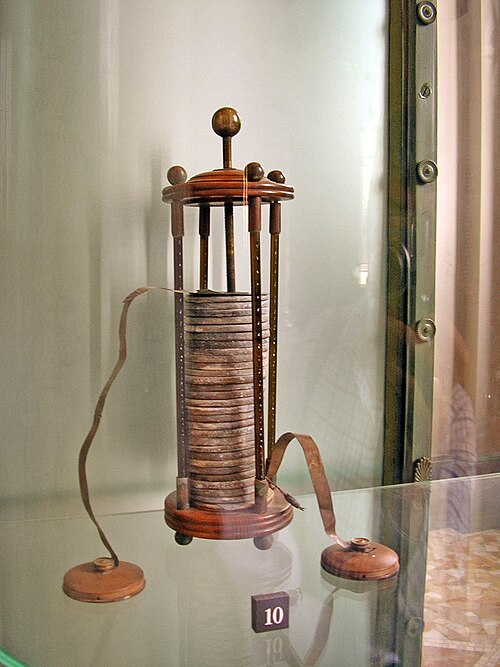
\includegraphics[width=\linewidth]{images/book3/volta-pile.jpg}
\end{minipage}\hfill
\begin{minipage}[t]{0.69\linewidth}
\vspace{0pt}
1800 में अलेस्सान्द्रो वोल्टा ने दो भिन्न धातुओं, ज़िंक और ताँबा या चाँदी, की
चकतियों का एक स्तंभ वर्णित किया, जो लवण-जल में भीगे कपड़े से अलग थीं: स्थिर
विद्युत धारा का पहला स्रोत। कुछ ही सप्ताहों में दूसरों ने उससे जल का अपघटन
किया, और एक दशक के भीतर हम्फ़्री डेवी ने एक बड़े पुंज से सोडियम और पोटैशियम को
उनके पिघले हाइड्रॉक्साइडों के \omterm{def:b2:batteries-electrolysis:electrolysis}{विद्युत-अपघटन} द्वारा पृथक कर लिया। छायाचित्र में
वोल्टा का अपना एक पुंज है। (छायाचित्र: गुइडोबी, CC BY-SA 3.0, विकिमीडिया
कॉमन्स।)
\end{minipage}
\end{history}

\section{ईंधन सेल}

\begin{definition}[ईंधन सेल]\label{def:b2:batteries-electrolysis:fuel-cell}
\emph{ईंधन सेल}\index{ईंधन सेल} ऐसा सेल है जिसके अभिकर्मक, एक ईंधन और एक
ऑक्सीकारक (प्रायः वायु की ऑक्सीजन), उसके इलेक्ट्रोडों तक लगातार पहुँचाए जाते हैं
और जिसके उत्पाद हटाए जाते हैं, ताकि वह तब तक धारा देता रहे जब तक
उसे आपूर्ति मिलती रहे।
\end{definition}

\cref{ch:b2:cell-thermodynamics} की बस के प्रोटॉन-विनिमय झिल्ली सेल में
हाइड्रोजन प्लैटिनम उत्प्रेरक पर ऑक्सीकृत होती है,
\ce{H2 -> 2H+ + 2e-}, प्रोटॉन एक पतली अम्लीय बहुलक झिल्ली को पार करते हैं, और ऑक्सीजन
दूसरी ओर अपचित होती है, \ce{O2 + 4H+ + 4e- -> 2H2O}। प्लैटिनम पर हाइड्रोजन
का ऑक्सीकरण एक \omterm{def:b2:current-potential-curves:fast-slow}{तीव्र निकाय} है; ऑक्सीजन का अपचयन हर इलेक्ट्रोड पर
मंद है। उत्क्रमणीय सेल के \qty{1.23}{V} और कार्य-वोल्टता के बीच खोई वोल्टता का
अधिकांश भाग ऑक्सीजन इलेक्ट्रोड का \omterm{def:b2:current-potential-curves:overpotential}{अधिविभव} है,
शेष झिल्ली का प्रतिरोध और, उच्च धारा पर, उत्प्रेरक तक ऑक्सीजन की
आपूर्ति (एक \omterm{def:b2:current-potential-curves:limiting-current}{सीमांत धारा})।

\section{विद्युत-अपघटन}

\begin{definition}[विद्युत-अपघटन]\label{def:b2:batteries-electrolysis:electrolysis}
\emph{विद्युत-अपघटन}\index{विद्युत-अपघटन} एक अस्वतः रेडॉक्स अभिक्रिया है
जिसे बाह्य जनित्र द्वारा दी गई धारा से बलपूर्वक चलाया जाता है; जिस सेल में यह
होती है वह \emph{विद्युत-अपघटक}\index{विद्युत-अपघटक} है। ऐनोड, जहाँ
ऑक्सीकरण होता है, जनित्र के धनात्मक ध्रुव से जुड़ा होता है।
\end{definition}

\begin{proposition}[ऊष्मागतिक न्यूनतम वोल्टता]\label{prop:b2:batteries-electrolysis:minimum-voltage}
जिस \omterm{def:b2:batteries-electrolysis:electrolysis}{विद्युत-अपघटन} की अभिक्रिया के लिए $\Delta_r G > 0$ है, उसे कम से कम
$\Delta_r G/(nF)$ की वोल्टता चाहिए।
\end{proposition}

\begin{proof}
जनित्र प्रति मोल अभिक्रिया कार्य $nFU$ देता है; उलटी अभिक्रिया पर लागू
\cref{thm:b2:cell-thermodynamics:delta-g-nfe} से प्राप्त विद्युत कार्य कम से कम
$\Delta_r G$ होना चाहिए।
\end{proof}

\begin{proposition}[विद्युत-अपघटक की वोल्टता]\label{prop:b2:batteries-electrolysis:electrolysis-voltage}
धारा $I$ प्रवाहित करने वाले \omterm{def:b2:batteries-electrolysis:electrolysis}{विद्युत-अपघटक} को चाहिए:
\[
  U = (E_a - E_c) + \eta_a + |\eta_c| + rI ,
\]
जहाँ $E_a$, $E_c$ ऐनोड और कैथोड युग्मों के साम्य विभव हैं
($E_a - E_c = \Delta_r G/(nF)$), $\eta_a$, $\eta_c$ उस धारा पर उनके \omterm{def:b2:current-potential-curves:overpotential}{अधिविभव}
और $r$ इलेक्ट्रोडों के बीच का प्रतिरोध।
\end{proposition}

\begin{proof}
सेल की तरह, वही धारा ऐनोड पर ऐनोडी है, विभव $E_a +
\eta_a$ पर, और कैथोड पर कैथोडी, $E_c + \eta_c$ पर; जनित्र को उसे
विद्युत-अपघट्य से भी गुज़ारना होता है, जिससे $rI$ जुड़ता है।
\end{proof}

\begin{method}[विद्युत-अपघटन का पूर्वानुमान]\label{met:b2:batteries-electrolysis:predict-electrolysis}
\begin{enumerate}
  \item ऐनोड पर ऑक्सीकृत हो सकने वाली हर स्पीशीज़ (ऐनोड धातु और
        विलायक सहित) और कैथोड पर अपचित हो सकने वाली हर स्पीशीज़ (विलायक सहित)
        सूचीबद्ध कीजिए।
  \item प्रयुक्त इलेक्ट्रोड पदार्थों पर उनके \omterm{def:b2:current-potential-curves:ie-curve}{धारा--विभव वक्र} खींचिए।
  \item वोल्टता बढ़ाने पर जिस पहले ऐनोडी वक्र और पहले कैथोडी
        वक्र तक पहुँचा जाता है, वे अभिक्रियाएँ देते हैं; बड़ी धाराओं पर अगले वक्र
        अपनी धाराएँ जोड़ते हैं।
\end{enumerate}
\end{method}

\begin{definition}[फ़ैराडे दक्षता]\label{def:b2:batteries-electrolysis:faradaic-efficiency}
\omterm{def:b2:batteries-electrolysis:electrolysis}{विद्युत-अपघटन} की \emph{फ़ैराडे दक्षता}\index{फ़ैराडे दक्षता} $\eta_F$ प्रवाहित आवेश का
वह अंश है जो वांछित उत्पाद बनाता है। उसकी \emph{विशिष्ट ऊर्जा खपत}\index{विशिष्ट ऊर्जा खपत}
उत्पाद के प्रति इकाई द्रव्यमान प्रयुक्त विद्युत ऊर्जा है।
\end{definition}

\begin{proposition}[फ़ैराडे का नियम]\label{prop:b2:batteries-electrolysis:faraday-mass}
धारा $I$, जो समय $t$ तक \omterm{def:b2:batteries-electrolysis:faradaic-efficiency}{फ़ैराडे दक्षता} $\eta_F$ के साथ प्रवाहित की जाए,
द्रव्यमान $m = \eta_F MIt/(nF)$ का ऐसा उत्पाद बनाती है जिसका मोलर द्रव्यमान $M$
है और जो प्रति मोल $n$ इलेक्ट्रॉनों से बनता है।
\end{proposition}

\begin{proof}
आवेश $It$, जिसका $\eta_F It$ उत्पाद बनाता है,
\cref{prop:b2:cell-thermodynamics:charge} से $\eta_F It/(nF)$ मोल के संगत है।
\end{proof}

\begin{proposition}[प्रति किलोग्राम ऊर्जा]\label{prop:b2:batteries-electrolysis:energy}
वोल्टता $U$ और \omterm{def:b2:batteries-electrolysis:faradaic-efficiency}{फ़ैराडे दक्षता} $\eta_F$ पर \omterm{def:b2:batteries-electrolysis:faradaic-efficiency}{विशिष्ट ऊर्जा
खपत} $w = nFU/(\eta_F M)$ है।
\end{proposition}

\begin{proof}
ऊर्जा $UIt$ है और द्रव्यमान $\eta_F MIt/(nF)$; भाग दीजिए।
\end{proof}

\section{औद्योगिक विद्युत-अपघटन}

\paragraph{ज़िंक।} अधिकांश ज़िंक \cref{ch:b2:ellingham} के अम्लीय ज़िंक सल्फ़ेट
विलयन के \omterm{def:b2:batteries-electrolysis:electrolysis}{विद्युत-अपघटन} से प्राप्त होता है। ज़िंक कैथोड पर जमता है, यद्यपि
\ce{H+} प्रबलतर ऑक्सीकारक है: ज़िंक पर \ce{H+} का अपचयन अत्यंत मंद है,
और ज़िंक तरंग तक पहले पहुँचा जाता है; ऐनोड ऑक्सीजन छोड़ता है।

\begin{omfigure}
\begin{tikzpicture}
\begin{axis}[omie, width=0.82\linewidth, height=5.6cm, xmin=-1.6, xmax=2.4,
  ymin=-2.4, ymax=2.4, xlabel={$E$ (V)}, ylabel={$i$}, clip=true, clip mode=individual]
\addplot[omcathodic] table[x=E, y=i] {figdata/out/bachelor-2-ie-curves-g-cath.dat};
\addplot[omanodic] table[x=E, y=i] {figdata/out/bachelor-2-ie-curves-g-an.dat};
\draw[densely dotted] (axis cs:-0.76,-2.2) -- (axis cs:-0.76,0.4);
\draw[densely dotted] (axis cs:0,-2.2) -- (axis cs:0,0.4);
\node[font=\scriptsize, anchor=south] at (axis cs:-0.76,0.4) {$-0.76$};
\node[font=\scriptsize, anchor=south east] at (axis cs:-0.02,0.4) {$0$};
\node[font=\scriptsize, omDef, anchor=north west, align=left] at (axis cs:-0.7,-1.05) {\ce{Zn^2+} $\to$ \ce{Zn},\\ पठार};
\node[font=\scriptsize, omDef, anchor=east, align=right] at (axis cs:-1.32,-0.9) {\ce{H+} $\to$ \ce{H2}\\ Zn पर};
\node[font=\scriptsize, omThm, anchor=east] at (axis cs:1.85,1.6) {\ce{H2O} $\to$ \ce{O2}};
\node[font=\scriptsize, gray, align=center] at (axis cs:-0.38,-0.5) {यहाँ ज़िंक पर\\ कोई \ce{H2} नहीं};
\end{axis}
\end{tikzpicture}

{\small ज़िंक कैथोड के साथ अम्लीय ज़िंक सल्फ़ेट विलयन का \omterm{def:b2:batteries-electrolysis:electrolysis}{विद्युत-अपघटन}
(मॉडल वक्र)। यद्यपि \ce{H+}/\ce{H2} युग्म ($\qty{0}{V}$)
\ce{Zn^2+}/\ce{Zn} ($\qty{-0.76}{V}$) से ऊपर है, ज़िंक पर \ce{H+} का अपचयन
लगभग \qty{-1.1}{V} से पहले आरंभ नहीं होता: इनके बीच केवल ज़िंक जमता है।
ऐनोड पर जल ऑक्सीजन में ऑक्सीकृत होता है।}
\end{omfigure}

\paragraph{क्लोरीन और सोडियम हाइड्रॉक्साइड।} लवण-जल का \omterm{def:b2:batteries-electrolysis:electrolysis}{विद्युत-अपघटन} ऐसे सेल में किया जाता है
जो केवल धनायनों को गुज़रने देने वाली झिल्ली से विभाजित है। ऐनोड पर क्लोराइड
ऑक्सीकृत होता है, \ce{2Cl- -> Cl2 + 2e-}; कैथोड पर जल अपचित होता है, \ce{2H2O +
2e- -> H2 + 2OH-}; आवेश संतुलित करने के लिए सोडियम आयन झिल्ली पार करते हैं, और
क्लोराइड-मुक्त सोडियम हाइड्रॉक्साइड विलयन कैथोड वाली ओर से निकलता है। मानक
परिस्थितियों में \ce{2Cl- + 2H2O -> Cl2 +
H2 + 2OH-} के लिए ऊष्मागतिक न्यूनतम $\Delta_r G/(2F) = \qty{2.19}{V}$ है। ऐनोड पर
ऑक्सीजन के बजाय क्लोरीन बनती है, यद्यपि \ce{O2}/\ce{H2O} युग्म नीचे है: प्रयुक्त ऐनोड
पदार्थों पर जल का ऑक्सीकरण दोनों में अधिक मंद है।
% ledger: dfg:OH-_ao, dfg:Cl-_ao, dfg:H2O_l

\begin{omfigure}
\begin{tikzpicture}[font=\small, >={Stealth}]
  \draw[thick] (0,0) rectangle (6,3.4);
  \draw[thick, dashed, omProp] (3,0) -- (3,3.4);
  \fill[black!30] (0.4,0.3) rectangle (0.7,3.0);
  \fill[black!50] (5.3,0.3) rectangle (5.6,3.0);
  \node[font=\scriptsize] at (0.55,3.3) {$+$};
  \node[font=\scriptsize] at (5.45,3.3) {$-$};
  \node[font=\scriptsize, align=center] at (1.85,1.9) {लवण-जल\\ \ce{2Cl-} $\to$\\ \ce{Cl2 + 2e-}};
  \node[font=\scriptsize, align=center] at (4.2,1.9) {\ce{NaOH}\\ विलयन\\ \ce{2H2O + 2e-} $\to$\\ \ce{H2 + 2OH-}};
  \draw[->, thick, omDef] (2.6,0.8) -- (3.4,0.8) node[pos=0.1, above, font=\scriptsize] {\ce{Na+}};
  \draw[->, thick] (1.0,3.4) -- (1.0,4.0) node[above] {\ce{Cl2}};
  \draw[->, thick] (5.0,3.4) -- (5.0,4.0) node[above] {\ce{H2}};
  \draw[->, thick] (-0.8,0.6) -- (0,0.6) node[pos=0, left] {लवण-जल प्रवेश};
  \draw[->, thick] (6,0.6) -- (6.8,0.6) node[right] {\ce{NaOH} निकास};
  \node[font=\scriptsize, omProp, anchor=north] at (3,-0.05) {धनायन-विनिमय झिल्ली};
\end{tikzpicture}

{\small झिल्ली वाला क्लोर-क्षार सेल, व्यवस्था-रूप। केवल सोडियम आयन
झिल्ली पार करते हैं, इसलिए कैथोड पर बना हाइड्रॉक्साइड क्लोरीन से नहीं मिलता।}
\end{omfigure}

\paragraph{ऐलुमिनियम।} ऐलुमिनियम ऑक्साइड को पिघले क्रायोलाइट,
\ce{Na3AlF6}, में घोला जाता है, जो ऐलुमिना से कहीं नीचे पिघलता है, और उसका \omterm{def:b2:batteries-electrolysis:electrolysis}{विद्युत-अपघटन}
एक कार्बन कैथोड, जिस पर द्रव ऐलुमिनियम जमा होता है, और कार्बन ऐनोडों के बीच किया जाता है जो
कार्बन डाइऑक्साइड के रूप में जल जाते हैं (हॉल--हेरू प्रक्रम):
\[
  \ce{2Al2O3 + 3C -> 4Al + 3CO2} .
\]
लगभग \qty{1250}{K} पर ऊष्मागतिक न्यूनतम लगभग \qty{1.18}{V} है
(\cref{pb:b2:batteries-electrolysis:1}); उस समस्या का सेल इसके साढ़े तीन गुने पर
काम करता है, और अतिरिक्त ऊर्जा उस ऊष्मा में बदलती है जो कुंड को
पिघला हुआ रखती है।

\begin{omfigure}
\begin{tikzpicture}[font=\small, >={Stealth}]
  \draw[thick, fill=black!12] (0,0) rectangle (7,3.2);
  \fill[black!45] (0.3,0.3) rectangle (6.7,0.8);
  \fill[gray!35] (0.3,0.8) rectangle (6.7,1.4);
  \fill[orange!30] (0.3,1.4) rectangle (6.7,2.5);
  \foreach \x in {1.0,3.0,5.0} {
    \fill[black!75] (\x,1.75) rectangle (\x+1.0,3.6);
    \draw[thick] (\x+0.5,3.6) -- (\x+0.5,4.2);
  }
  \draw[thick] (1.5,4.2) -- (5.5,4.2) node[right] {$+$};
  \node[font=\scriptsize, align=left, anchor=west] at (7.3,2.6) {कार्बन ऐनोड, \ce{CO2} में जलते हुए};
  \node[font=\scriptsize, align=left, anchor=west] at (7.3,1.95) {पिघला क्रायोलाइट + घुला \ce{Al2O3}};
  \node[font=\scriptsize, align=left, anchor=west] at (7.3,1.1) {द्रव ऐलुमिनियम (कैथोड)};
  \node[font=\scriptsize, align=left, anchor=west] at (7.3,0.55) {कार्बन कैथोड खंड, $-$};
  \draw[densely dotted] (6.7,2.6) -- (7.3,2.6) (6.7,1.95) -- (7.3,1.95) (6.7,1.1) -- (7.3,1.1) (6.7,0.55) -- (7.3,0.55);
\end{tikzpicture}

{\small हॉल--हेरू सेल, अनुप्रस्थ काट, व्यवस्था-रूप। ऐलुमिनियम द्रव धातु के कुंड
की सतह पर अपचित होता है, जो कैथोड का कार्य करता है; ऑक्साइड आयन
कार्बन ऐनोडों पर विसर्जित होते हैं, जिन्हें वे कार्बन डाइऑक्साइड में जला देते हैं।}
\end{omfigure}

\begin{history}[हॉल और हेरू, 1886]
\begin{minipage}[t]{0.18\linewidth}
\vspace{0pt}
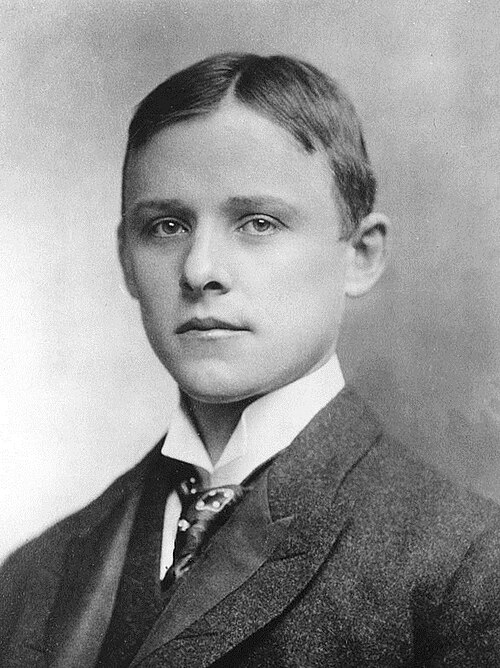
\includegraphics[width=\linewidth]{images/book3/hall.jpg}
\end{minipage}\hspace{0.02\linewidth}%
\begin{minipage}[t]{0.18\linewidth}
\vspace{0pt}
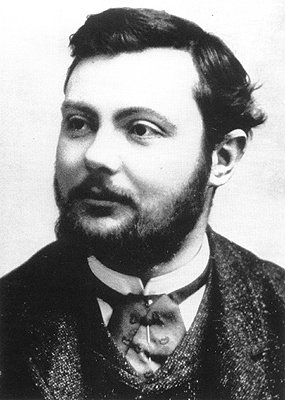
\includegraphics[width=\linewidth]{images/book3/heroult.jpg}
\end{minipage}\hfill
\begin{minipage}[t]{0.58\linewidth}
\vspace{0pt}
1886 में, बाईस या तेईस वर्ष की आयु में, चार्ल्स मार्टिन हॉल और
पॉल हेरू ने, अटलांटिक के दोनों ओर, स्वतंत्र रूप से पाया कि ऐलुमिना
पिघले क्रायोलाइट में घुलती है और वहाँ उसका \omterm{def:b2:batteries-electrolysis:electrolysis}{विद्युत-अपघटन} किया जा सकता है। ऐलुमिनियम, जो तब तक
सोडियम द्वारा उसके क्लोराइड के अपचयन से बनने वाली एक बहुमूल्य धातु था,
बिजली के बड़े पैमाने पर उत्पादन के बाद हल्की धातुओं में सबसे सस्ता बन गया।
(चित्र: हॉल, लगभग 1880 का दशक, अज्ञात लेखक, सार्वजनिक अधिकार-क्षेत्र; हेरू,
सार्वजनिक अधिकार-क्षेत्र; विकिमीडिया कॉमन्स।)
\end{minipage}
\end{history}

\paragraph{सोडियम।} सोडियम जल से जमाया नहीं जा सकता, जिसका वह अपचयन कर देता है।
यह पिघले सोडियम क्लोराइड के \omterm{def:b2:batteries-electrolysis:electrolysis}{विद्युत-अपघटन} से बनाया जाता है, जिसका गलनांक
एक मिलाए गए लवण से घटाया जाता है (\omterm{def:b2:solid-liquid-diagrams:eutectic}{गलनक्रांतिक मिश्रण}, \cref{ch:b2:solid-liquid-diagrams}),
और उपोत्पाद क्लोरीन होती है। \qty{1100}{K} पर $\Delta_f G^\circ(\ce{NaCl}, \text{l}) =
\qty{-310.7}{kJ/mol}$: न्यूनतम वोल्टता \qty{3.22}{V} है।
% ledger: janafG:NaCl.1100

\section{अभ्यास}

\begin{exercise}[$\star$]\label{exo:b2:batteries-electrolysis:1}
अम्ल में ज़िंक वाले चित्र पर अकेले ज़िंक और ताँबे को छूते ज़िंक का \omterm{def:b2:batteries-electrolysis:mixed-potential}{मिश्र विभव} और
धारा (मॉडल इकाइयाँ) पढ़िए, और बताइए कि कौन
तेज़ी से घुलता है।
\end{exercise}

\begin{exercise}[$\star$]\label{exo:b2:batteries-electrolysis:2}
100~\% \omterm{def:b2:batteries-electrolysis:faradaic-efficiency}{फ़ैराडे दक्षता} के साथ \qty{500}{A} की धारा द्वारा एक घंटे में ज़िंक का
कितना द्रव्यमान जमता है?
\end{exercise}

\begin{exercise}[$\star$]\label{exo:b2:batteries-electrolysis:3}
अध्याय में दी गई गिब्स संभवन ऊर्जाओं से सीसा--अम्ल \omterm{def:b2:batteries-electrolysis:battery}{संचायक} की मानक
वोल्टता, और \qty{12}{V} की कार बैटरी में सेलों की संख्या
परिकलित कीजिए।
\end{exercise}

\begin{exercise}[$\star$]\label{exo:b2:batteries-electrolysis:4}
यदि एक ग्राम लिथियम पूरा \ce{Li+} में ऑक्सीकृत हो जाए, तो वह ऐम्पियर-घंटों में
कितना आवेश दे सकता है?
\end{exercise}

\begin{exercise}[$\star\star$]\label{exo:b2:batteries-electrolysis:5}
ताँबे का एक शोधन सेल \qty{24}{h} तक \qty{200}{A} प्रवाहित करता है और
\qty{5.50}{kg} ताँबा जमाता है। \omterm{def:b2:batteries-electrolysis:faradaic-efficiency}{फ़ैराडे दक्षता} परिकलित कीजिए।
\end{exercise}

\begin{exercise}[$\star\star$]\label{exo:b2:batteries-electrolysis:6}
ज़िंक का एक विद्युत-निष्कर्षण सेल \qty{3.3}{V} पर 90~\% की \omterm{def:b2:batteries-electrolysis:faradaic-efficiency}{फ़ैराडे दक्षता} के साथ काम करता है
(अभ्यास के आँकड़े)। प्रति किलोग्राम ज़िंक विद्युत ऊर्जा परिकलित कीजिए।
\end{exercise}

\begin{exercise}[$\star\star$]\label{exo:b2:batteries-electrolysis:7}
एक बैटरी \qty{0.10}{A} पर \qty{1.55}{V} और \qty{0.60}{A} पर \qty{1.40}{V} देती है।
\omterm{def:b2:current-potential-curves:overpotential}{अधिविभवों} को नगण्य मानकर उसका आंतरिक प्रतिरोध और बिना धारा के
उसकी वोल्टता ज्ञात कीजिए।
\end{exercise}

\begin{exercise}[$\star\star$]\label{exo:b2:batteries-electrolysis:8}
झिल्ली सेल में लवण-जल का \omterm{def:b2:batteries-electrolysis:electrolysis}{विद्युत-अपघटन} किया जाता है। इलेक्ट्रोड अभिक्रियाएँ लिखिए,
न्यूनतम वोल्टता परिकलित कीजिए, और समझाइए कि उत्पादों को अलग क्यों रखना
चाहिए।
\end{exercise}

\begin{exercise}[$\star\star$]\label{exo:b2:batteries-electrolysis:9}
\qty{1100}{K} पर पिघले सोडियम क्लोराइड के \omterm{def:b2:batteries-electrolysis:electrolysis}{विद्युत-अपघटन} के लिए न्यूनतम वोल्टता और
प्रति किलोग्राम सोडियम न्यूनतम ऊर्जा परिकलित कीजिए।
\end{exercise}

\begin{exercise}[$\star\star\star$]\label{exo:b2:batteries-electrolysis:10}
\omterm{def:b2:current-potential-curves:ie-curve}{धारा--विभव वक्रों} से समझाइए कि ज़िंक कैथोड पर अम्लीय कुंड से ज़िंक का लेपन क्यों
किया जा सकता है, और पूर्वानुमान दीजिए कि लेपन के आरंभ में प्लैटिनम कैथोड पर
क्या होगा।
\end{exercise}

\begin{exercise}[$\star\star\star$]\label{exo:b2:batteries-electrolysis:11}
\qty{1100}{K} और \qty{1300}{K} पर $\Delta_f G^\circ$ ($\ce{Al2O3}$: $-1328.3$ और
$-1262.3$; $\ce{CO2}$: $-396.0$ और $-396.2$ \unit{kJ/mol}) से \qty{1250}{K} पर हॉल--हेरू
सेल की न्यूनतम वोल्टता परिकलित कीजिए, और उसकी तुलना ऐसे अक्रिय ऐनोड से कीजिए
जिस पर ऑक्सीजन मुक्त होती।
\end{exercise}

\begin{exercise}[$\star\star\star$]\label{exo:b2:batteries-electrolysis:12}
बिजली को जल के \qty{1.80}{V} पर \omterm{def:b2:batteries-electrolysis:electrolysis}{विद्युत-अपघटन} द्वारा संचित किया जाता है और
\qty{0.70}{V} पर \omterm{def:b2:batteries-electrolysis:fuel-cell}{ईंधन सेल} में पुनः प्राप्त किया जाता है, दोनों 100~\% \omterm{def:b2:batteries-electrolysis:faradaic-efficiency}{फ़ैराडे दक्षता} के साथ।
पूर्ण-चक्र दक्षता परिकलित कीजिए और समझाइए कि ऊर्जा कहाँ जाती है।
\end{exercise}

\section{समस्या: एक टन ऐलुमिनियम}

\begin{problem}[{सप्ताहांत समस्या --- हॉल--हेरू सेल की अभिक्रिया
और उसकी न्यूनतम वोल्टता, एक टन ऐलुमिनियम बनाने के लिए आवेश और समय,
प्रयुक्त ऊर्जा, और जला हुआ कार्बन}]
\label{pb:b2:batteries-electrolysis:1}
आँकड़े: \qty{1100}{K} और \qty{1300}{K} पर JANAF गिब्स संभवन ऊर्जाएँ
(\unit{kJ/mol}): \ce{Al2O3} $-1328.3$, $-1262.3$; \ce{CO2} $-396.0$, $-396.2$। सेल
(अभ्यास के आँकड़े): धारा \qty{300}{kA}, वोल्टता \qty{4.1}{V}, \omterm{def:b2:batteries-electrolysis:faradaic-efficiency}{फ़ैराडे दक्षता}
94~\%, कुंड लगभग \qty{1250}{K} पर। मोलर द्रव्यमान (\unit{g/mol}): Al 26.982, C 12.011,
O 15.999। ऐलुमिनियम को \qty{298}{K} से उसके गलनांक पर द्रव तक लाने की
ऊष्मा: \qty{28.69}{kJ/mol}।
% ledger: janafG:Al2O3.1100, janafG:Al2O3.1300, janafG:CO2.1100, janafG:CO2.1300, aw:Al, aw:C, aw:O, hT:Al_l.933, const:F

\medskip
\noindent\textbf{भाग I --- न्यूनतम वोल्टता।}
\begin{enumerate}
  \item अभिकारकों और उत्पादों में ऐलुमिनियम, ऑक्सीजन और कार्बन की ऑक्सीकरण संख्याएँ
        दीजिए।
  \item कैथोड और ऐनोड अर्ध-अभिक्रियाएँ लिखिए, पिघले कुंड द्वारा ले जाए गए ऑक्साइड आयन
        \ce{O^2-} के साथ।
  \item समग्र अभिक्रिया और विनिमित इलेक्ट्रॉनों की संख्या $n$ लिखिए।
  \item \qty{1250}{K} पर \ce{Al2O3} और \ce{CO2} के $\Delta_f G^\circ$ का अंतर्वेशन कीजिए।
  \item \qty{1250}{K} पर $\Delta_r G^\circ$ परिकलित कीजिए।
  \item न्यूनतम वोल्टता निकालिए।
  \item अक्रिय ऐनोड के साथ न्यूनतम वोल्टता परिकलित कीजिए,
        \ce{2Al2O3 -> 4Al + 3O2}, और कार्बन की भूमिका समझाइए।
\end{enumerate}

\medskip
\noindent\textbf{भाग II --- आवेश और समय।}
\begin{enumerate}[resume]
  \item एक टन में ऐलुमिनियम की कितनी मात्रा है?
  \item 100~\% \omterm{def:b2:batteries-electrolysis:faradaic-efficiency}{फ़ैराडे दक्षता} के साथ इसे कितना आवेश चाहिए?
  \item वास्तव में कितना आवेश प्रवाहित होता है?
  \item एक सेल को एक टन बनाने में कितना समय लगता है?
  \item एक सेल प्रति दिन ऐलुमिनियम का कितना द्रव्यमान बनाता है?
  \item सुझाइए कि आवेश का खोया हुआ 6~\% कहाँ जाता है।
\end{enumerate}

\medskip
\noindent\textbf{भाग III --- ऊर्जा।}
\begin{enumerate}[resume]
  \item प्रति टन विद्युत ऊर्जा परिकलित कीजिए।
  \item इसे \unit{kW.h} प्रति किलोग्राम में व्यक्त कीजिए।
  \item न्यूनतम वोल्टता और 100~\% दक्षता पर प्रति किलोग्राम न्यूनतम ऊर्जा
        परिकलित कीजिए।
  \item शेष ऊर्जा कहाँ जाती है, और वह पूरी तरह व्यर्थ
        क्यों नहीं है?
  \item एक सेल की विद्युत शक्ति परिकलित कीजिए।
  \item एक किलोग्राम कबाड़ को फिर से पिघलाने के लिए आवश्यक ऊष्मा,
        \unit{kW.h} में, परिकलित कीजिए और तुलना कीजिए।
  \item कार्य-वोल्टता का कितना अंश ऊष्मागतिक न्यूनतम है?
\end{enumerate}

\medskip
\noindent\textbf{भाग IV --- कार्बन।}
\begin{enumerate}[resume]
  \item समीकरण के अनुसार प्रति टन ऐलुमिनियम जले कार्बन का द्रव्यमान
        परिकलित कीजिए।
  \item प्रति टन ऐनोडों द्वारा मुक्त कार्बन डाइऑक्साइड का द्रव्यमान परिकलित कीजिए।
  \item वास्तविक सेल इससे अधिक कार्बन जलाते हैं। दो कारण सुझाइए।
  \item ऐनोड \ce{CO2} को प्रति किलोग्राम ऐलुमिनियम व्यक्त कीजिए।
  \item अक्रिय ऐनोड वोल्टता के लिए और मुक्त गैस के लिए
        क्या बदलेगा?
  \item प्रति किलोग्राम ऐलुमिनियम विद्युत ऊर्जा बताइए।
\end{enumerate}
\end{problem}
